\newpage
\section{Boltzmann Machines and RBMs}

\subsection{Before BMs\cite{rojas1996hopfield, hopfield, coursera_nn}}

\subsubsection{General RNNs}
In early 1980-x general \textbf{recurrent neural networks} (RNNs), described by (general) \emph{asyclic} graph began to arise.
\begin{itemize}
\item     mostly binary units, $\{0, 1\}$ (or $\{-1, 1\}$);
\gooditem signal feedback $\Rightarrow$ \textbf{memory} compared to FF NNs (more specifically, \emph{content-addressable memory} (CAM) $\Leftrightarrow$ weights themselves are used to store patterns);
\baditem  in general if activations are non-linear function they are hard to train (oscillations and chaotic behavior).
\end{itemize}

\begin{figure}[h]
\begin{mdframed}
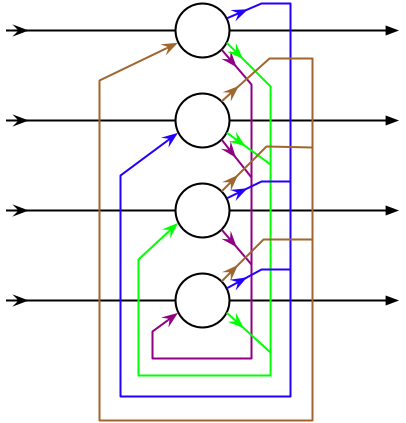
\includegraphics[scale=0.4]{img/general_rnn.png}
\centering
\caption{Example architecture of RNN}
\label{fig:general_rnn}
\end{mdframed}
\end{figure}

\vspace{1em}
\subsubsection{Hopfield Nets}
Later in $\approx$1982 John Hopfield has shown that if RNN has symmetric weights ($W_{ij}=W_{ji}$), and has no self-loops ($W_{ii}=0$), network's dynamics \textbf{is guaranteed} to converge to some stationary state. Fully-connected variant (complete graph) of such a network is called a \emph{Hopfield Network}.

Moreover, he also shown that each state of the Hopfield Net is associated with a scalar value referred to as the \emph{energy} of the network ($s_{i}\in\{-1, 1\}$ -- state of i-th neuron, $b_{i}$ -- bias of i-th neuron ($-b_{i}$ is activation threshold for the unit)):
\begin{align}
E = -\frac{1}{2}\sum_{i,j}W_{ij}s_is_j-\sum_{i}b_is_i=\commenttwo{$W_{ij}=W_{ji}$,}{$W_{ii}=0$} = -\sum_{i<j}W_{ij}s_is_j-\sum_{i}b_is_i
\end{align}
and local minima of $E(\mathbf{s};\mathbf{W}, \mathbf{b})\;\Leftrightarrow\;$ stable configurations of network. It is the first example of so-called \textbf{energy-based model}. Learning algorithm for such a model alter its (global) energy function to achieve desired properties. For instance, if a Hopfield Net is trained as autoassociator, the goal of learning is to shape energy function in such a way, that its local minima correspond to training examples (= patterns to "remember").
\begin{figure}[h]
\begin{mdframed}
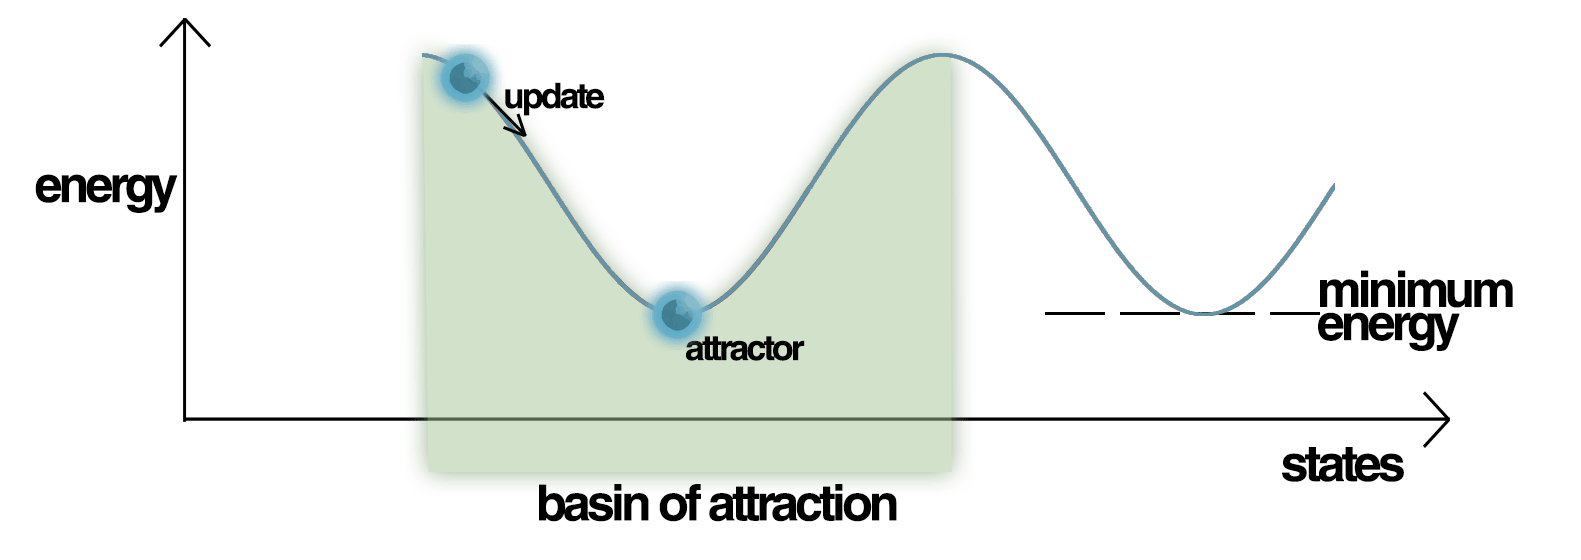
\includegraphics[scale=0.2]{img/energy_landscape.png}
\centering
\caption{Energy Landscape of a Hopfield Network, highlighting the current state of the network (up the hill), an attractor state to which it will eventually converge, a minimum energy level and a basin of attraction shaded in green. Note how the update of the Hopfield Network is always going down in Energy.}
\label{fig:energy_landscape}
\end{mdframed}
\end{figure}

\vspace{1em}
\subsubsection{Learning algorithms for Hopfield Nets}
There are exist couple of learning algorithms for Hopfield Nets.
First, thanks to simple quadratic shape of $E$, it is straightforward to calculate how i-th neuron influences the global energy:
\begin{gather*}
\Delta E_i = E(\mathbf{s}|s_i=\text{off}) - E(\mathbf{s}|s_i=\text{on}) = E(\mathbf{s}|s_i=0) - E(\mathbf{s}|s_i=1) =\\= -\sum_{k<j}W_{kj}s_ks_j\evalat{s_i=0} -\sum_{j}b_js_j\evalat{s_i=0}  + \sum_{k<j}W_{kj}s_ks_j\evalat{s_i=1} + \sum_{j}b_js_j\evalat{s_i=1} =\\=
\underbrace{-\l( \sum_{k<j, k \neq i, j \neq i}W_{kj}s_ks_j + \sum_{j \neq i}b_js_j \r) + \l( \sum_{k<j, k \neq i, j \neq i}W_{kj}s_ks_j + \sum_{j \neq i}b_js_j \r)}_{=0} +
\underbrace{\sum_{j<i}W_{ji}s_j}_{k=i} + \underbrace{\sum_{i<k}W_{ik}s_k}_{j=i} + b_i =\\= \comment{$W_{ij}=W_{ji}$, $W_{jj}=0$} = \sum_jW_{ij}s_is_j + b_i
\end{gather*}
This lead to the learning algorithm called \textbf{Binary Threshold Decision Rule} (BTDR):
\begin{itemize}
\item Randomly initialize states (or to desired pattern if want CAM);
\item While not converged or for fixed number of iterations:
	\subitem For each neuron:
		\subsubitem Change its state if this will decrease global energy. More specifically:
		 $$
		 s_i \leftarrow
		 \begin{cases}
		 +1,  \;\;\Delta E_i > 0,\\
		 s_i, \;\;\Delta E_i = 0,\\
		 -1,  \;\;\Delta E_i < 0.\\
		 \end{cases}
		 $$
\end{itemize}
This learning algorithm is \emph{local} and \emph{incremental}, thus biologically plausible. Also neurons could have been updated simultaneously, but it is less likely that there is exists "global clock" in biological system, and such kind of updates can also cause oscillation or chaotic behavior.

One important \underline{drawback} of such an algorithm, is that once we stuck in poor local minimum, we cannot escape it, it is also one of the reasons why Boltzmann Machines was more successful.

\vspace{2em}
Another learning algorithm is based on famous \textbf{Hebb rule}: "Cells that fire together, wire together". In the simplest case it simply says:
\begin{gather}
W_{ij} \leftarrow x_ix_j,
\end{gather}
where $\mathbf{x}=\{x_1 \ldots x_N\}$ is binary input pattern. If $x_i$ and $x_j$ are the same, then $W_{ij}$ is positive thus i-th and j-th state tend to become equal. Opposite happens when $x_i$ and $x_j$ are different. Now one can show that network's dynamics will be the same if
\begin{gather}
W_{ij} \leftarrow \frac{1}{N}x_ix_j
\end{gather}
If we need to remember not 1 but $P$ patterns, sum corresponding update for each pattern (for each pattern pretend there are no others):		
\begin{gather}
W_{ij} \leftarrow \frac{1}{N}\sum_{p=1}^Px_i^{(p)}x_j^{(p)}
\end{gather}
This way network will act as CAM, see Fig. \ref{fig:hopfield}. The network will converge to a "remembered" state if it is given only part of the state $\Rightarrow$ can be used to recover from a distorted input to the trained state that is most similar to the input.
\begin{figure}[h]
\begin{mdframed}
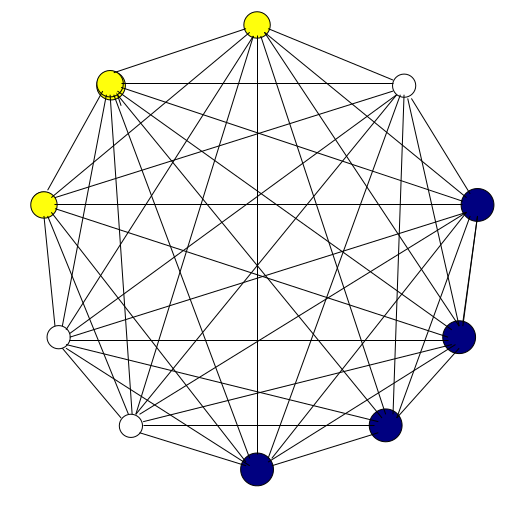
\includegraphics[scale=0.4]{img/hopfield.png}
\centering
\caption{A Hopfield network as an autoassociator. One enters a pattern in
blue nodes and let the network evolve. After a while one reads out the yellow
nodes. The memory of the Hopfield network associates the yellow node pattern
with the blue node pattern.}
\label{fig:hopfield}
\end{mdframed}
\end{figure}

\vspace{1em}
For instance, train Hopfield net such that $(1, -1, 1, -1, 1)$ is a local minimum of $E$ (phase 1 -- memorization). Next, if the network is properly trained, it can recover $(1, -1, 1, -1, 1)$ from $(1, -1, \mathbf{-1}, -1, 1)$ input (phase 2 -- recognition). Hopfield nets can be used for denoising of simple fonts.	

\vspace{1em}
Many generalizations of this rule exist, but fundamentally Hopfield nets had quite some drawbacks (even for binary data):
\begin{itemize}
\baditem patterns are stored in the network itself, thus can be intractable for large $N$;
\baditem capacity, one can reliably store only $P << N$ patterns;
\baditem spurious minima, poor local minima;
\baditem no probabilistic interpretation.
\end{itemize}
But anyway Hopfield Nets and energy-based models played a big role in development of deep learning and now we proceed to the one of the most famous modification of Hopfield Net -- Boltzmann Machine.

\subsection{Boltzmann Machines\cite{coursera_nn, aarts1988simulated, fischer2012introduction, tutorial2014lisa}}
\subsubsection{Main ideas}
Boltzmann Machine (developed $\approx$1980-85 by G. Hinton) is a \emph{stochastic}, \emph{generative} counter-part of Hopfield Nets. From PGM point of view, it is an example of MRF (undirected graphical model). It is also an example of Ising model.
\\[1em]
Two main ideas:
\begin{enumerate}
\item Instead of storing "memories" in stable configurations of Hopfield net, use them for "interpretation" of the input data. Thus, all units are divided into 2 groups: \emph{visible} and \emph{hidden} (see Fig. \ref{fig:bm}).
\begin{figure}[h]
\begin{mdframed}
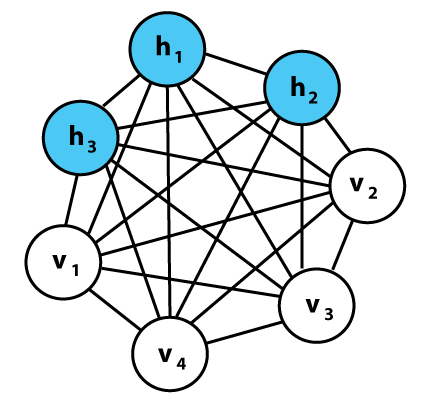
\includegraphics[scale=0.4]{img/bm.png}
\centering
\caption{A graphical representation of an example Boltzmann machine. Each undirected edge represents dependency. In this example there are 3 hidden units and 4 visible units. This is not a restricted Boltzmann machine.}
\label{fig:bm}
\end{mdframed}
\end{figure}

\item To escape local minima, assume units are \emph{Gibbs distibuted} with the same energy function (1) and use more advanced learning algorithms (see below).
\end{enumerate}

\subsubsection{Historical development and informal explanation}
Inspired from statistical physics, assume that units' states are Gibbs distributed (= Boltzmann distributed) random variables for global energy (1) $\;\Rightarrow\;$ energy of the state is proportional to the negative log-probability of that state and also the following identity holds:
\begin{gather}
\Delta E_i = E(\mathbf{s}|s_i=0) - E(\mathbf{s}|s_i=1) \;\propto\; -k_BT\log p\{s_i=0\}+k_BT\log p\{s_i=1\},
\end{gather}
By absorbing Boltzmann's constant $k_B$ into introduced notion of (artificial) temperature $T$ ($T\leftarrow k_BT$) ($\Leftrightarrow$ by considering \emph{dimensionless} units where $k_B=1$) , we can rearrange equation (5) and solve for $ p\{s_i=1\}$. We will obtain so-called \emph{normal logistic equation}:
\begin{gather}
 p\{s_i=1\}=\frac{1}{1+\exp\l(-\frac{\Delta E_i}{T}\r)}=\text{sigm}\l(-\frac{\Delta E_i}{T}\r)
\end{gather} 
We obtained a \textbf{Modified BTDR}:
\begin{itemize}
\item Randomly initialize states;
\item In cycle for each unit if its state reversal will yield energy decrease, reverse its state with probability described by (6).
\end{itemize}
After running for long enough time at certain $T$, it turns out that probability of a global state of network will \emph{depend only upon global state's energy}, and not on the initial state (in accordance with Boltzmann distribution). 
\\$\Rightarrow$ Distribution of all possible configurations (global states) converges to same \emph{stationary distribution} (this state in physics is called thermal equilibrium). Note that being in thermal equilibrium, system does not necessary is in the state of the lowest energy, which still might be oscillating, \textbf{but} if we start running the network from a high temperature, and gradually decrease it over time until we reach a thermal equilibrium at low $T$, we may converge to a distribution where the energy level fluctuates around the global minimum (at least this can happen with higher probability than in Hopfield Nets). 
\\This process is called \textbf{simulated annealing}. Yes, it seems like development of BMs gave fundament to one of the most famous and successful algorithms of global optimization.
\\[1em]
Now if we want to train the network so that the chance it will converge to a global state is according to an external distribution (e.g. data) that we have over these states, we need to \emph{set the weights} so that the global states with the highest probabilities will get the lowest energies. By altering parameters we can shape the distribution produced by BM using (6), it is the main idea of Boltzmann machine.
\\[1em]
BM is interpreted in the following way. Visible units provide open interface to the world and represent data. Hidden units represent hidden patterns in the data. Usually it is trained by using maximum likelihood estimation using approximate (why see below) gradient ascent. It is also equivalent \cite{goodfellow2016deep} to minimizing KL-divergence between external distribution (which is usually empirical data distribution) and model distribution produced by the network.

\subsubsection{More formal derivations}
\u{Notations}:
\\$\mathbf{v}\in\{0,1\}^D=\{0,1\}^V$ -- vector of visible units,
\\$\mathbf{h}\in\{0,1\}^H$ -- vector of hidden units,

Energy of a particular state $(\mathbf{v},\mathbf{h})$ is:
\begin{gather}
E(\mathbf{v},\mathbf{h};\bs{\psi})=-\frac{1}{2}\mb{v}^T\mb{L}\mb{v}-\frac{1}{2}\mb{h}^T\mb{J}\mb{h}-\mb{v}^T\mb{W}\mb{h}-\mb{b}^T\mb{v}-\mb{c}^T\mb{h},
\end{gather}
it is nothing else but (1) with old $\mb{W}$ split into $\mb{L}$ describing vis-vis weights, $\mb{J}$ describing hid-hid weights, and new $\mb{W}$ describing vis-hid connections, and the same for biases. The reason is to keep notations consistent with later parts where we will get rid of $\mb{L}$ and $\mb{J}$. Of course, $\mb{L}$ and $\mb{J}$ are symmetric with zeros on the main diagonal. $\bs{\psi}=\{\mb{L},\mb{J},\mb{W},\mb{b},\mb{c}\}$ are model parameters.

Probability of the configuration $(\mb{v},\mb{h})$ is (according to the Boltzmann distribution):
\begin{gather}
p(\mathbf{v},\mathbf{h};\bs{\psi})=\frac{e^{-E(\mathbf{v},\mathbf{h};\bs{\psi})}}{\sum_{\mb{\t{v}},\mb{\t{h}}} e^{-E(\mathbf{\t{v}},\mathbf{\t{h}};\bs{\psi})} }=:\frac{p^*(\mb{v},\mb{h}; \bs{\psi})}{Z(\bs{\psi})},
\end{gather}
where $p^*(\mb{v},\mb{h}; \bs{\psi})$ is unnormalized probability of the configuration and $Z(\bs{\psi})$ is a normalizer also called \emph{partition function}.
\\$\Rightarrow$
\\Probability that model assigns to a visible vector $\mb{v}$ is
\begin{gather}
p(\mb{v};\bs{\psi})=\sum_{\mb{h}}p(\mathbf{v},\mathbf{h};\bs{\psi})=:\frac{e^{-\mathcal{F}(\mb{v};\bs{\psi})}}{\sum_{\mb{\t{v}}} e^{-\mathcal{F}(\mb{\t{v}};\bs{\psi})} },
\end{gather}
where
\begin{gather}
\mc{F}(\mb{v};\bs{\psi})=-\log\l( \sum_{\mb{h}}e^{-E(\mb{v},\mb{h};\bs{\psi})} \r)
\end{gather}
is called \emph{free energy} (\emph{free} because all the hidden states are marginalized out; the name is inspired again from physics), useful quantity which will be used later.
\\[1em]
\u{Now lets calculate} $p(v_i=1|\mb{h},\mb{v}_{-i})$: (omit $\bs{\psi}$ for brevity)

\begin{empheq}[box={\mybox[1em][1em]}]{gather*}
p(v_i=1|\mb{h},\mb{v}_{-i})=\frac{p(v_i=1,\mb{v}_{-i},\mb{h})}{p(\mb{v}_{-i},\mb{h})}=
\frac{p(v_i=1,\mb{v}_{-i},\mb{h})}{p(v_i=0,\mb{v}_{-i},\mb{h})+p(v_i=1,\mb{v}_{-i},\mb{h})}
\\=\frac{e^{-E(v_i=1,\mb{v}_{-i},\mb{h})}}{e^{-E(v_i=0,\mb{v}_{-i},\mb{h})} + e^{-E(v_i=1,\mb{v}_{-i},\mb{h})}}=\frac{1}{1+e^{-\l[E(v_i=0,\ldots)-E(v_i=1,\ldots)\r]}}=\text{sigm}\l[E(v_i=0,\ldots)-E(v_i=1,\ldots)\r]=
\\=\comment{$E(\mb{v},\mb{h})=-\sum_{j<k}L_{jk}v_jv_k -\sum_{l<m}J_{lm}h_lh_m -\sum_{j,l}W_{jl}v_jh_l-\sum_jb_jv_j-\sum_lc_lh_l $}=
\\=\comment{sums w/o $v_i$ (2nd, 5th) cancel out}=\text{sigm}\l[\underbrace{-\ldots+\sum_{j<k,j\neq i, k\neq i}L_{jk}v_jv_k}_{=0}+\underbrace{\sum_{i<k}L_{ik}v_k}_{j=i}+ \underbrace{\sum_{j<i}L_{ji}v_j}_{k=i} -\r.\\\l.\underbrace{-\ldots+\sum_{j\neq i, l}W_{jl}v_jh_l}_{=0}+  \underbrace{\sum_lW_{il}h_l}_{j=i}+b_i\r]=\comment{$L_{ij}=L_{ji}, L_{ii}=0$}=\text{sigm}\l[ \sum_lW_{il}h_l+\sum_kL_{ik}v_k+b_i \r]
\end{empheq}	
So:
\begin{gather}
\boxed{p(v_i=1|\mb{h},\mb{v}_{-i})=\text{sigm}\l( \sum_kL_{ik}v_k+\sum_lW_{il}h_l+b_i \r)}
\end{gather}
\u{Symmetrically},
\begin{gather}
\boxed{p(h_j=1|\mb{v},\mb{h}_{-j})=\text{sigm}\l( \sum_lJ_{jl}h_l+\sum_iW_{ij}v_i+c_j \r)}
\end{gather}
\\[1em]
\u{Maximum Likelihood learning}
\\Suppose we have dataset $\mc{D}=\{\mb{x}_1,\ldots\mb{x}_N\}, \mb{x}_n\in\{0,1\}^D$. The goal is to maximize $\sum_{n=1}^N\log p(\mb{x}_n;\bs{\psi})$ for parameters $\bs{\psi}$. For a single training example $\mb{v}$ and any parameter $\theta$:
\begin{empheq}[box={\mybox[1em][1em]}]{gather*}
\frac{\partial}{\partial\theta}\log p(\mb{v};\bs{\psi})=
\frac{\partial}{\partial\theta}\l(\log \sum_{\mb{h}}e^{-E(\mb{v},\mb{h};\bs{\psi})}-
\log\sum_{\mb{\t{v}},\mb{\t{h}}}e^{-E(\mb{\t{v}},\mb{\t{h}};\bs{\psi})} \r)=
\\=-\frac{1}{\sum_{\mb{h}}e^{-E(\mb{v},\mb{h};\bs{\psi})}}\sum_{\mb{h}}\l[e^{-E(\mb{v},\mb{h};\bs{\psi})} \cdot \frac{\partial}{\partial\theta}E(\mb{v},\mb{h};\bs{\psi}) \r]+
\frac{1}{\sum_{\mb{\t{v}},\mb{\t{h}}}e^{-E(\mb{\t{v}},\mb{\t{h}};\bs{\psi})}}
\sum_{\mb{\t{v}},\mb{\t{h}}}\l[e^{-E(\mb{\t{v}},\mb{\t{h}};\bs{\psi})}\cdot \frac{\partial}{\partial\theta} E(\mb{\t{v}},\mb{\t{h}};\bs{\psi}) \r]=
\\=\comment{$\frac{e^{-E(\mb{v},\mb{h};\bs{\psi})}}{\sum_{\mb{h}}e^{-E(\mb{v},\mb{h};\bs{\psi})}}=\frac{\frac{1}{Z(\theta)}e^{-E(\mb{v},\mb{h};\bs{\psi})}}{\frac{1}{Z(\theta)}\sum_{\mb{h}}e^{-E(\mb{v},\mb{h};\bs{\psi})}}=\frac{p(\mb{h},\mb{v};\bs{\psi})}{p(\mb{v};\bs{\psi})}=p(\mb{h}|\mb{v};\bs{\psi})$}=
\\=-\underbrace{\sum_{\mb{h}}p(\mb{h}|\mb{v};\bs{\psi})\cdot\frac{\partial}{\partial\theta}E(\mb{v},\mb{h};\bs{\psi})}_{\E_{\mb{h}|\mb{v};\bs{\psi}}\l[\frac{\partial}{\partial\theta}E(\mb{v},\mb{h};\bs{\psi})\r]}
+\underbrace{\sum_{\mb{\t{v}},\mb{\t{h}}}p(\mb{\t{v}},\mb{\t{h}};\bs{\psi})\cdot\frac{\partial}{\partial\theta}E(\mb{\t{v}},\mb{\t{h}};\bs{\psi})}_{\E_{\mb{\t{v}},\mb{\t{h}};\bs{\psi}}\l[\frac{\partial}{\partial\theta}E(\mb{\t{v}},\mb{\t{h}};\bs{\psi})\r]}
\end{empheq}
This we obtain
\begin{gather}
\boxed{\frac{\partial}{\partial\theta}\log p(\mb{v};\bs{\psi})=-\E_{\mb{h}|\mb{v};\bs{\psi}}\l[\frac{\partial E}{\partial\theta}(\mb{v},\mb{h};\bs{\psi})\r]+\E_{\mb{\t{v}},\mb{\t{h}};\bs{\psi}}\l[\frac{\partial E}{\partial\theta}(\mb{\t{v}},\mb{\t{h}};\bs{\psi})\r]}
\end{gather}
And avegared over all data points:
\begin{gather}
\frac{1}{N}\sum_{n=1}^N \frac{\partial}{\partial\theta} \log p(\mb{x}_n;\bs{\psi})=-\frac{1}{N}\sum_{n=1}^N \E_{\mb{h}|\mb{v};\bs{\psi}}\l[\frac{\partial E}{\partial\theta}(\mb{x}_n,\mb{h};\bs{\psi})\r] + \E_{\mb{\t{v}},\mb{\t{h}};\bs{\psi}}\l[\frac{\partial E}{\partial\theta}(\mb{\t{v}},\mb{\t{h}};\bs{\psi})\r]
\end{gather}
or solely in terms of expectations:
\begin{gather}
\boxed{\E_{\mb{v}\sim P_{\text{data}}(\mb{v})}\l[ \frac{\partial}{\partial\theta}\log p(\mb{v};\bs{\psi}) \r]=-\E_{\mb{v},\mb{h}\sim P_{\text{data}}(\mb{v},\mb{h};\bs{\psi})}\l[ \frac{\partial E}{\partial\theta}(\mb{v},\mb{h};\bs{\psi}) \r] + \E_{\mb{v},\mb{h}\sim P_{\text{model}}(\mb{v},\mb{h};\bs{\psi})}\l[ \frac{\partial E}{\partial\theta}(\mb{v},\mb{h};\bs{\psi}) \r]}
\end{gather}
where $P_{\text{data}}(\mb{v})=\frac{1}{N}\sum_{n=1}^N \delta_{\mb{v},\mb{x}_n}$ is \emph{empirical distribution}, $P_{\text{data}}(\mb{v},\mb{h};\bs{\psi})=p(\mb{h}|\mb{v};\bs{\psi})P_{\text{data}}(\mb{v})$ is \emph{complete-data distribution} and $P_{\text{model}}$ is a distribution modelled by BM.
\\[1em]
Before we move on, there is one more equivalent form of gradient of data log-likelihood:
\begin{gather}
-\frac{\partial}{\partial\theta}\log p(\mb{v};\bs{\psi})=\frac{\partial}{\partial\theta}\mc{F}(\mb{v})-\sum_{\mb{\t{v}}}p(\mb{\t{v}})\frac{\partial}{\partial\theta}\mc{F}(\mb{\t{v}})
\end{gather}
Notice that the above gradient contains two terms, which are referred to as the \textbf{positive} and \textbf{negative} phase. The terms positive and negative do not refer to the sign of each term in the equation, but rather reflect their effect on the probability density defined by the model. The first term increases the probability of training data (by reducing the corresponding free energy), while the second term decreases the probability of samples generated by the model.
\\[1em]
\u{Derivatives of the energy w.r.t. model parameters}:
$$
E(\mathbf{v},\mathbf{h};\bs{\psi})=-\frac{1}{2}\mb{v}^T\mb{L}\mb{v}-\frac{1}{2}\mb{h}^T\mb{J}\mb{h}-\mb{v}^T\mb{W}\mb{h}-\mb{b}^T\mb{v}-\mb{c}^T\mb{h},
$$
\begin{itemize}
\item $\frac{\partial E}{\partial \mb{L}}=-\mb{v}\mb{v}^T$ (remember that $\mb{L}$ is symmetric)
\item Similarly $\frac{\partial E}{\partial \mb{J}}=-\mb{h}\mb{h}^T$ and $\frac{\partial E}{\partial \mb{W}}=-\mb{v}\mb{h}^T$
\item Finally $\frac{\partial E}{\partial \mb{b}}=-\mb{v}$ and $\frac{\partial E}{\partial \mb{c}}=-\mb{h}$
\end{itemize}
So 1 update of the weights $\mb{W}$ using vanilla gradient ascent looks like:
\begin{align}
\mb{g}_{\mb{W}} &\;\leftarrow\; \E_{\mb{v},\mb{h}\sim P_{\text{data}}(\mb{v},\mb{h};\bs{\psi})}\l[\mb{v}\mb{h}^T\r]-\E_{\mb{v},\mb{h}\sim P_{\text{model}}(\mb{v},\mb{h};\bs{\psi})}\l[\mb{v}\mb{h}^T\r]
\\ 
\mb{W} &\;\leftarrow\; \mb{W} + \alpha\cdot\mb{g}_{\mb{W}}
\end{align}
and similarly for other parameters.
\\[1em]
\u{Problems}
\\
So far it seems like everything is ok, but there is 1 very serious problem, \textbf{both expectations in (13) $\Leftrightarrow$ (15) are simply intractable}. First sum has $O\l(2^H\r)$ terms while the second one has $O\l(2^{V+H}\r)$ terms. Moreover, even $p(\mb{h}|\mb{v};\bs{\psi})$ or $p(\mb{v},\mb{h};\bs{\psi})$ are intractable because of partition function in denominators which itself has exponentially many in $V+H$ terms.
\\[1em]To overcome this computational burden, G. Hinton and T. Sejnowski in 1983 proposed algorithm that uses Gibbs sampling to approximate both expectations. The idea is that both expectations are approximated by states of 2 Markov chains (Monte-Carlo sampling), which are updated using Gibbs sampling $\forall$ training example during training.
\\[1em]The main problem with the last algorithm is \tb{time} required to approach distribution, especially when estimating the model's expectations, since the Gibbs chain may need to explore a highly multimodal energy landscape + exponential in machine size and magnitude of weights time to collect equilibrium statistics. We will see that in RBM Gibbs sampling can be performed much more efficiently thus having much more efficient learning algorithm.
\\[1em]
To summarize, Boltzmann Machines is a Monte Carlo version of Hopfield Net with discrimination between visible and hidden units and that uses annealed Gibbs sampling. Boltzmann Machines were one of the first neural networks capable of learning internal representations, and are able to represent and (given sufficient time) solve difficult combinatoric problems + they are again are considered a biologically plausiable because during learning only local information is used, i.e. the update for a particular weight connecting two units depend only on the statistics of those two units (this can be seen by considering equation (17) element-wisely).
\subsubsection{Additional facts}
\textbullet{} from formulae (11),(12) we can see that probability of one unit being on is given by a linear model (logistic regression) from the values of the other units.
\\
\textbullet{} in the presence of hidden units, BM becomes a \emph{universal approximator} in a sense that it can learn arbitraty point mass function over discrete variables (without hidden units it could have learned only linear relationships between variables) \cite{goodfellow2016deep}
\\
\textbullet{} it is also interesting that in this model we can compute $p(\mb{h}|\mb{v};\bs{\psi})$ exactly and efficiently, unlike many other models with hidden variables like VAE etc., and still this model can learn fairly complex distributions (+ previous bullet)

\subsection{Restricted Boltzmann Machines\cite{coursera_nn, fischer2012introduction, tutorial2014lisa, hinton2010practical, fischer2014training, smolensky1986information, gibbs_wiki}}
\subsubsection{Intro and comparison with general BM}
A \emph{restricted Boltzmann machine} was invented by P. Smolensky in 1986 and is characterized by absense of hid-hid and vis-vis connections (see Fig. \ref{fig:rbm}).
\begin{figure}[h]
\begin{mdframed}
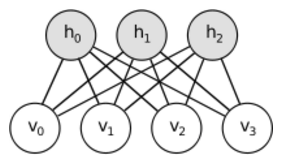
\includegraphics[scale=0.5]{img/rbm.png}
\centering
\caption{Diagram of a restricted Boltzmann machine with four visible units and three hidden units (no bias units).}
\label{fig:rbm}
\end{mdframed}
\end{figure}
In this case we have $\mb{L}=\mb{J}=\mb{0}$ and the energy function for RBM simplifies:
\bg
E(\mathbf{v},\mathbf{h};\bs{\psi})=-\mb{v}^T\mb{W}\mb{h}-\mb{b}^T\mb{v}-\mb{c}^T\mb{h}
\eg
Because of the \emph{bipartite} structure of the graph, in this MRF \tb{all hidden units are conditionally independent given visible ones and vice versa} ($\bs{\psi}$ is omitted for brevity):
\bg
p(\mb{h}|\mb{v})=\prod_jp(h_j|\mb{v}), \;\;\; p(\mb{v}|\mb{h})=\prod_ip(v_i|\mb{h})
\eg
(Formally every path in this graphical model between different $h_j$ and $h_l$ is blocked by $\mb{v}$ and vice versa).
\\[1em]
Taking this into account, formulae (11) and (12) simplify too:
\bg
p(v_i=1|\mb{h})=\text{sigm}\l( \sum_lW_{il}h_l+b_i \r),
\\
p(h_j=1|\mb{v})=\text{sigm}\l( \sum_iW_{ij}v_i+c_j \r)	
\eg
very important that each of these formulae can be computed \tb{in parallel}:
\bg
p(\mb{v}=\mb{1}|\mb{h})=\text{sigm}\l( \mb{W}\mb{h}+\mb{b} \r),
\\
p(\mb{h}=\mb{1}|\mb{v})=\text{sigm}\l( \mb{W}^T\mb{v}+\mb{c} \r)	
\eg
this makes exact inference tractable (as opposed to general BM).
\\[1em]
It is also easier to calculate marginalized distribution of the visible variables (see Fig. \ref{fig:prod_experts})
\begin{figure}[h]
\begin{mdframed}
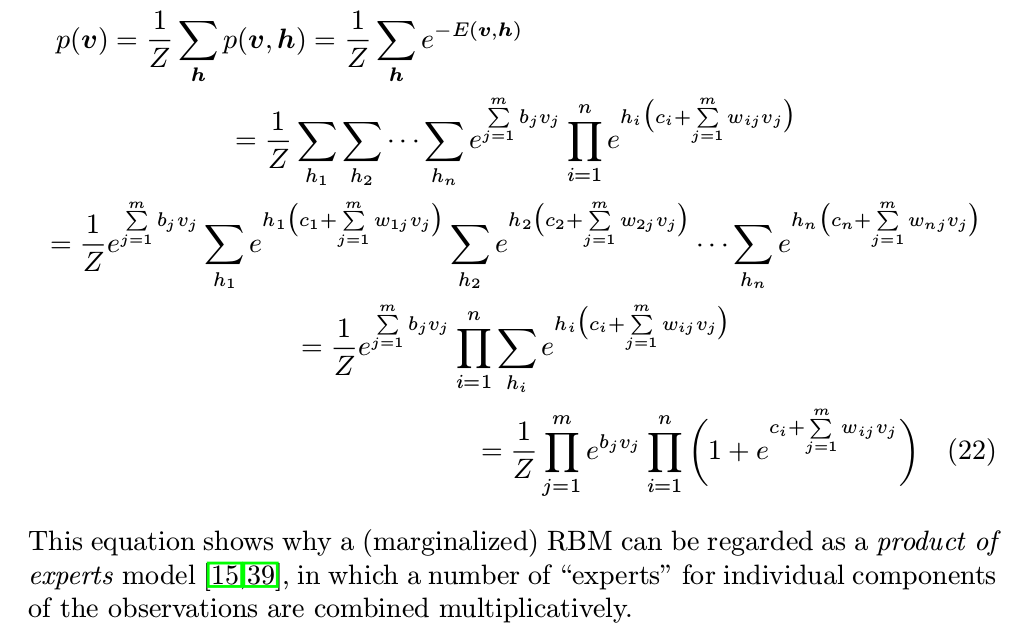
\includegraphics[scale=0.4]{formulae/prod_experts.png}
\centering
\caption{$p(\mb{v})$}
\label{fig:prod_experts}
\end{mdframed}
\end{figure}
\\[1em]
\u{Gradient of Log-Likelihood}
\\Recall
$$
\frac{\partial}{\partial\theta}\log p(\mb{v};\bs{\psi})=
-\sum_{\mb{h}}p(\mb{h}|\mb{v};\bs{\psi})\cdot\frac{\partial}{\partial\theta}E(\mb{v},\mb{h};\bs{\psi})
+\sum_{\mb{\t{v}},\mb{\t{h}}}p(\mb{\t{v}},\mb{\t{h}};\bs{\psi})\cdot\frac{\partial}{\partial\theta}E(\mb{\t{v}},\mb{\t{h}};\bs{\psi})
$$
First term for $\theta=W_{ij}$ (omit $\bs{\psi}$):
\begin{empheq}[box={\mybox[1em][1em]}]{gather*}
[1]=-\sum_{\mb{h}} \prod_kp(h_k|\mb{v}) \cdot\frac{\partial}{\partial W_{ij}}E(\mb{v},\mb{h})=\comment{$\frac{\partial}{\partial W_{ij}}E(\mb{v},\mb{h})=-v_ih_j$}=\sum_{\mb{h}} \prod_kp(h_k|\mb{v})v_ih_j=
\\=\sum_{h_j}\sum_{\mb{h}_{-j}}p(h_j|\mb{v})p(\mb{h}_{-j}|\mb{v})h_jv_i=
\sum_{h_j\in\{0,1\}}h_jp(h_j|\mb{v})v_i \underbrace{\sum_{\mb{h}_{-j}}p(\mb{h}_{-j}|\mb{v})}_{=1}=p(h_j=1|\mb{v})\cdot v_i
\end{empheq}
The second term
$$
[2]=\sum_{\mb{\t{v}},\mb{\t{h}}}p(\mb{\t{v}},\mb{\t{h}})\cdot\frac{\partial}{\partial\theta}E(\mb{\t{v}},\mb{\t{h}})=\sum_{\mb{\t{v}}}p(\mb{\t{v}})\l(\sum_{\mb{\t{h}}}p(\mb{\t{h}}|\mb{\t{v}})\cdot\frac{\partial}{\partial\theta}E(\mb{\t{v}},\mb{\t{h}})\r)
$$
and thus can be computed in the same manner.
\\Eventually we obtain the following expressions for log-likelihood gradients:
\begin{align}
\frac{\partial}{\partial W_{ij}}\log p(\mb{v};\bs{\psi}) &= p(h_j=1|\mb{v})\cdot v_i
-\sum_{\mb{\t{v}}}p(\mb{\t{v}})\cdot p(h_j=1|\mb{\t{v}})\cdot \t{v}_i
\\
\frac{\partial}{\partial b_{i}}\log p(\mb{v};\bs{\psi}) &= v_i -\sum_{\mb{\t{v}}}p(\mb{\t{v}}) \cdot \t{v}_i
\\
\frac{\partial}{\partial c_{j}}\log p(\mb{v};\bs{\psi}) &= p(h_j=1|\mb{v}) - \sum_{\mb{\t{v}}}p(\mb{\t{v}}) \cdot p(h_j=1|\mb{\t{v}})
\end{align}
+ use formulae (21), (22). Averaged over all training examples, these formulae can also be rewritten in terms of expectations. Note that $\sum_{\mb{\t{v}}} p(\mb{\t{v}})[\cdots]=\E_{\mb{\t{v}}\sim P_{\text{\text{model}}}}[\cdots]$.
\\[1em]
Despite of the sound simplification and reducing of computational complexity because of the nice factorization, (25) - (27) are still intractable for regular RBMs because of the second terms which are exponential in $\min\{V, H\}$ (if $H<V$ we can factorize $p(\mb{v},\mb{h})=p(\mb{h})p(\mb{v}|\mb{h})$).
\\[1em]Thus, to avoid this complexity, we will approximate expectations by samples from the model distribution using MCMC-based algorithm \emph{Contrastive Divergence} (described below).
\\[1em]
\u{Quick summary}
\begin{center}
\begin{tabular}{ |c|c|c| } 
\hline
& \tb{general BM} & \tb{RBM} \\
\hline
\tb{exact Maximum Likelihood learning} & \color{red}intractable & intractable$^{*}$ \\
\hline
\tb{inference} & \color{red}approximate & \color{green}exact \\
\hline
\end{tabular}
\end{center}
$^{*}$ -- learning still can be done efficiently using Contrastive Divergence.

\subsubsection{Contrastive Divergence algorithm and modifications}
All common training algorithms for RBMs approximate expectations in log-likelihood gradients (25) - (27) by only single sample from RBM and perform gradient ascent on these approximations. 
\\[1em]
Samples in RBM can be obtained by running a Markov chain to convergence, using Gibbs sampling as the transition operator. 
In general, Gibbs sampling of the joint of $N$ random variables $\bs{\xi}=(\xi_1\ldots\xi_N)$ is done through a sequence of $N$ sampling sub-steps of the form $\xi_i\sim p(\xi_i|\bs{\xi}_{-i})$. If done sequentially, one can show that these sub-steps define reversible Markov chain with desired invariant joint distribution.
\\[1em]
For RBMs, $\xi$ consists of the set of visible and hidden units. However, since they are conditionally independent, $p(v_i|\mb{h},\mb{v}_{-i})=p(v_i|\mb{h})$ and $p(h_j|\mb{v},\mb{h}_{-j})=p(h_j|\mb{v})$ one can perform \tb{block} Gibbs sampling (which is impossible in BM). In this setting, visible units are sampled simultaneously given fixed values of the hidden units. Similarly, hidden units are sampled simultaneously given the visibles. A step in the Markov chain is thus taken as follows:
\bg
\mb{h}^{(n+1)}\;\sim\;\text{Ber}(\text{sigm}\l( \mb{W}^T\mb{v}^{(n)}+\mb{c} \r)),
\\
\mb{v}^{(n+1)}\;\sim\;\text{Ber}(\text{sigm}\l( \mb{W}\mb{h}^{(n+1)}+\mb{b} \r))
\eg
Graphically:
\begin{figure}[h]
\begin{mdframed}
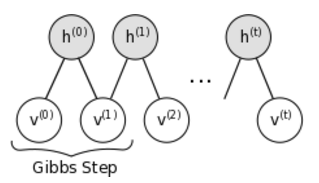
\includegraphics[scale=0.6]{img/gibbs.png}
\centering
\caption{Gibbs sampling in RBM.}
\label{fig:gibbs}
\end{mdframed}
\end{figure}
\\
As $n \rightarrow \infty$, samples $\left(\mb{v}^{(n)},\mb{h}^{(n)}\right)$ are guaranteed to be accurate samples of the model joint.
\\[1em]
In theory, each parameter update in the learning process would require running one such chain to convergence to obtain unbiased estimates of gradients of log-likelihood, which requires many sampling steps (prohibitively expensive) and moreover it is typically unclear for how long chain has to be run. As such, several algorithms have been devised for RBMs, in order to efficiently sample from.
\\[1em]
\u{Contrastive Divergence} (CD-k)
\\
This algorithm was proposed in 2002 by G.Hinton and uses two tricks to speed up the sampling process:
\begin{itemize}
\item since we eventually want $p_{\text{model}}(\mb{v}) \approx p_{\text{data}}(\mb{v})$ (Maximum Likelihood $\Leftrightarrow$ Minimizing KL divergence between $p_{\text{model}}$ and $p_{\text{data}}$ (empirical distribution)), \emph{we initialize the Markov chain with a training example}, so that the chain will be already close to having converged to its desired distribution.
\item CD does not wait for the chain to converge. Samples are obtained after only $k$-steps of Gibbs sampling. In practice, $k=1$ has been shown to work surprisingly well.
\end{itemize}
General formula for gradient approximation:
\bg
\frac{\partial}{\partial\theta}\log p(\mb{v}^{(0)};\bs{\psi})\approx 
-\sum_{\mb{h}}p(\mb{h}|\mb{v}^{(0)};\bs{\psi})\cdot\frac{\partial}{\partial\theta}E(\mb{v}^{(0)},\mb{h};\bs{\psi})
+\sum_{\mb{h}}p(\mb{h}|\mb{v}^{(k)};\bs{\psi})\cdot\frac{\partial}{\partial\theta}E(\mb{v}^{(k)},\mb{h};\bs{\psi})
\eg
Concrete formulae for gradient approximations:
\begin{align}
g_{W_{ij}} &\leftarrow p(h_j=1|\mb{v}^{(0)})\cdot v_i^{(0)}-p(h_j=1|\mb{v}^{(k)})\cdot v_i^{(k)}
\\
g_{b_i} &\leftarrow v_i^{(0)}-v_i^{(k)}
\\
g_{c_j} &\leftarrow p(h_j=1|\mb{v}^{(0)})-p(h_j=1|\mb{v}^{(k)})
\end{align}
with $\mb{v}^{(0)}:=\mb{v}$ -- training example
\\
Each gradient is a difference of the corresponding \tb{positive} and \tb{negative} gradients, see (16). It is thus described through sequence of \emph{positive phases}, where we clamp visible units to a particular state vector sampled from the training set $\mb{v}\leftarrow\mb{x}_i \sim p_{\text{data}}$, and \emph{negative phases}, where the network is run freely without fixing any states.
\\[0.5em]
\tb{Note}: originally formulae (31)-(33) should contain instead of $p(h_j=1|\mb{v})$ the samples of hidden units themselves (apart from sampling involved to estimate model's expectations), but stated variants typically provide slightly less noisy and thus faster learning, and it is not so important at all when RBM is used to pretrain hidden layer of units for DBN/DBM \cite{hinton2010practical}.
\\[1em]
Since $\mb{v}^{(k)}$ is not a sample from the stationary distribution the approximation the approximation (30) is biased. Obviously, as $k \rightarrow \infty$, bias vanishes. One can also show that CD does not maximize the likelihood of the data under the model, but minimize the difference of two KL-divergences:
\bg
D_{\text{KL}}(p_{\text{data}}(\mb{v})\;\|\;p_{\text{model}}(\mb{v}))-D_{\text{KL}}(p^{(k)}(\mb{v})\;\|\;p_{\text{model}}(\mb{v})),
\eg
where $p^{(k)}(\mb{v})$ is a distribution of visible variables after k steps of Markov chain. If chain already reached stationarity it holds that $p^{(k)}=p_{\text{model}} \;\Rightarrow\; D_{\text{KL}}(p^{(k)}(\mb{v})\;\|\;p_{\text{model}}(\mb{v}))=0$ and the approximation error of CD is vanishes.
\\[1em]
CD does not follow the gradient of any function \cite{hinton2010practical}.
\\[1em]
\u{Persistent CD}
In \cite{tieleman2008training} they rely on a single Markov chain, which has a persistent state (i.e., not restarting a chain for each observed example). For each parameter update, we extract new samples by simply running the chain for $k$-steps. The state of the chain is then preserved for subsequent updates. The general intuition is that if parameter updates are small enough compared to the mixing rate of the chain, the Markov chain should be able to "catch up" to changes in the model.
\\[1em]
Typically one uses as much markov chains as there are training examples in a minibatch. These persistent states of Markov chains can be used to generate samples after training. In \cite{hinton2010practical} they mention PCD learns significantly better models than CD-k for various k and is the recommended method if the aim is to build the best density model of the data. We will use a modification of PCD for DBM training.
\\[1em]
Also, recently the new algorithm \u{Parallel tempering} is proposed \cite{fischer2012introduction}. It introduces supplementary Gibbs chains that sample from more and more smoothed replicas of the original distribution. In the price of computational overhead it gives faster mixing Markov chain and thus less biased gradient approximation.
\subsubsection{Extensions}
\u{More general RBMs/BMs}
\\[1em]
So far we considered only case of binary (Bernoulli) both visible and hiddent units. But RBMs (and BMs) can also be extended to model $\R$-valued inputs/outputs. This can be achieved by altering the energy functio (more examples below). More generally RBM can be defined as any MRF (undirected graphical model) with conditionally independent visible units given hidden and vice versa and with energy function of the following kind:
\bg
E(\mb{v},\mb{h};\bs{\psi})=\sum_{i,j}\phi_{ij}(v_i,h_j;\bs{\psi})+\sum_i \omega_i(v_i;\bs{\psi}) + \sum_j \nu_j(h_j;\bs{\psi})
\eg
with $\R$-valued functions $\phi_{ij}, \omega_i, \nu_j$ for which partition function is finite $Z(\bs{\psi})<\infty$.
\\[1em]
\u{Conditional RBMs}
\\[1em]
some of the parameters in $E$ are replaced by parameterized functions of some conditioning random variables.
\\[1em]
\u{Classification RBMs (cRBMs)}
\\[1em]
In regular RBM we model $p(\mb{x})$. In classification RBM there are couple of choices:
\begin{itemize}
\item model $p(\mb{x},\mb{y})$ (\emph{generative mode})
\item model $p(\mb{y}|\mb{x})$ (\emph{discriminative mode}), equivalent to the above via Bayes theorem
\item $\alpha\cdot p(\mb{x},\mb{y})+(1-\alpha)\cdot p(\mb{y}|\mb{x})\rightarrow \text{max}$ (\emph{hybrid mode})
\end{itemize}
See more in \cite{hinton2010practical}.

\subsubsection{Different types of RBM units}
For a binary unit, the probability of turning on is given by the logistic sigmoid function of its total input, $x$.
\bg
p=\text{sigm}(x)=\frac{1}{1+e^{-x}}=\frac{e^x}{e^x+e^0}
\eg
The energy contributed by the unit is $-x$ if it is on and 0 if it is off. Equation (36) makes it clear that the probability of each of the two possible states is proportional to the negative exponential of its energy. This can be generalized to $K$ alternative states.
\\[1em]
\u{Softmax units}
\bg
p_j=\text{softmax}_j(\mb{x})=\frac{e^{x_j}}{\sum_{k=1}^K e^{x_k}}
\eg
It is the appropriate way to deal with a quantity that has $K$ alternative \emph{mutually exclusive} values which are not ordered in any way. When viewed in this way, the learning rule for the binary units in a softmax is identical to the rule for standard binary units.
\tb{The only difference is in the way the probabilities of the states are computed and the samples are taken} + Fig. \ref{fig:softmax_sampling}.
\\[0.5em]
Formally, for binary visible and softmax hidden: 
$$\mb{v}\in\{0,1\}^D,\mb{h}\in\text{One-hot}(H)=\l\{\mb{q}\in\{0,1\}^H \bigg| \sum_kq_k=1\r\}, H=K$$
Energy function has the same functional form, as for binary-binary RBM:
\bg
E(\mb{v},\mb{h};\bs{\psi})=-\sum_{j,l}W_{jl}v_jh_l-\sum_jb_jv_j-\sum_lc_lh_l
\eg
\\[1em]
\u{Multinomial units}
\\
Afurther generalization of the softmax unit is to sample $M$ times (with replacement) from the probability distribution instead of just sampling once. The $K$ different states can then have integer values bigger than 1, but the values must add to $M$. This is called a \emph{multinomial unit} and, again, the learning rule is unchanged. It is also equivalent \cite{hinton2009replicated} to $M$ softmax units with shared weights.
\\[0.5em]
Formally, for binary visible and multinomial hidden with $M$ samples: 
$$\mb{v}\in\{0,1\}^D,\t{\mb{h}}\in\l\{\mb{q}\in\{0,1,\ldots,M\}^H \bigg| \sum_kq_k=M\r\}, H=K$$
Energy function has the same functional form, as for binary-binary RBM:
\bg
E(\mb{v},\t{\mb{h}};\bs{\psi})=-\sum_{j,l}W_{jl}v_j\t{h}_l-\sum_jb_jv_j-\sum_lc_l\t{h}_l,
\eg
where $\t{h}_l=\sum_{m=1}^M h_l^{(m)}$ -- count for $l$-th discrete value of hidden units. Typically, this variant of RBM is used for topic modelling \cite{hinton2009replicated} (visible are Multinomial, hidden -- binary). Often $M$ is equal to $K$. In this case, it is also useful to scale hidden bias term by $M$, this will allow to behave sensible when deal with documents of the different lengths.
\\[1em]
\u{Gaussian visible units}
\\
To be able to model real-valued data $\mb{v}\in\R^D$, one solution is to replace the binary visible units by linear units with independent Gaussian noise. The energy function then becomes:
\bg
E(\mb{v},\mb{h};\bs{\psi})=\frac{1}{2}\sum_{i,j}\frac{(v_i-b_i)^2}{\sigma_i^2}-\sum_jc_jh_j-\sum_{i,j}W_{ij}\frac{v_i}{\sigma_i}h_j
\eg
where $\sigma_i$ is the standard deviation of the Gaussian noise for visible unit $i$. It is possible to learn the variance of the noise for each visible unit but this is difficult using CD-k. In many applications, it is much easier to first normalise each component of the data to have zero mean and unit variance and then to use noise free reconstructions, with the variance in equation (40) set to 1.
\\[1em]
From (38) one can derive formulae for activations \cite{salakhutdinov2013learning, krizhevsky2009learning}:
\bg
p(h_j=1|\mb{v})=\text{sigm}\l(\sum_iW_{ij}\frac{v_i}{\sigma_i}+c_j\r),
\\
v_i|\mb{h}\;\sim\;\mc{N}\l(\sigma_i\sum_jW_{ij}h_j+b_i;\;\sigma_i^2\r)=\sigma_i\sum_jW_{ij}h_j+b_i+\sigma_i\cdot\mc{N}(0; 1)
\eg
\\[1em]
There also exist other types of units, such as gaussian for both visible and hidden units, binomial units, rectifier linear units etc., but they more rarely used and are out of the scope of these notes. See more in \cite{hinton2010practical}.

\subsubsection{Free energies formulae}
\textbullet{} \u{Free energy for binary visible and hidden units (19)} (Similarly to Fig. \ref{fig:prod_experts}):
\begin{empheq}[box={\mybox[1em][1em]}]{gather*}
\mc{F}(\mb{v};\bs{\psi})=-\log\l( \sum_{\mb{h}}e^{-E(\mb{v},\mb{h};\bs{\psi})} \r)=
-\log \sum_{\mb{h}} \exp\l(\sum_{i,j}W_{ij}v_ih_j+\sum_ib_iv_i+\sum_jc_jh_j\r)=\\
=-\log \l[\exp\l(\sum_ib_iv_i\r)\cdot\sum_{\mb{h}} \exp\l(\sum_{i,j}W_{ij}v_ih_j+\sum_jc_jh_j\r)\r]=\\
=-\sum_ib_iv_i-\log \sum_{\mb{h}} \underbrace{\exp\l(\sum_jh_j\l(\sum_iW_{ij}v_i+c_j\r)\r)}_{\prod_j \exp\l(h_j\l(\sum_iW_{ij}v_i+c_j\r)\r)}=\comment{$\sum_{\mb{h}}\prod_j f_j(h_j)=\prod_j\sum_{h_j}f_j(h_j)$}=\\
=-\mb{b}\cdot\mb{v}-\sum_j \log\l( \underbrace{ \sum_{h_j\in\{0,1\}}\exp \l[h_i \sum_iW_{ij}v_i+c_j\r]}_{1+\exp\l(\sum_iW_{ij}v_i+c_j\r)}\r)
=-\mb{b}\cdot\mb{v}-\sum_j \text{softplus}\l(\sum_iW_{ij}v_i+c_j\r),
\end{empheq}
where $\text{softplus}(x):=\log(1+e^x)$.
\begin{gather}
\boxed{\mc{F}(\mb{v};\bs{\psi})=-\mb{b}\cdot\mb{v}-\sum_j \text{softplus}\l(\sum_iW_{ij}v_i+c_j\r)}
\end{gather}
\\[1em]
\textbullet{} \u{Free energy for Bernoulli-Softmax RBM (38)}:
\begin{empheq}[box={\mybox[1em][1em]}]{gather*}
\mc{F}(\mb{v};\bs{\psi})=-\log\l( \sum_{\mb{h}}e^{-E(\mb{v},\mb{h};\bs{\psi})} \r)=
-\sum_ib_iv_i-\log \sum_{\mb{h}} \underbrace{\exp\l(\sum_jh_j\l(\sum_iW_{ij}v_i+c_j\r)\r)}_{\prod_j \exp\l(h_j\l(\sum_iW_{ij}v_i+c_j\r)\r)}=\\
=-\mb{b}\cdot\mb{v}-\log \sum_{j=1}^K\exp\l(\sum_iW_{ij}v_i+c_j\r),
\end{empheq}
\begin{gather}
\boxed{\mc{F}(\mb{v};\bs{\psi})=-\mb{b}\cdot\mb{v}-\log \sum_{j=1}^K\exp\l(\sum_iW_{ij}v_i+c_j\r)}
\end{gather}
\\[1em]
\textbullet{} \u{Free energy for Bernoulli-Multinomial RBM (39)}:
\begin{empheq}[box={\mybox[1em][1em]}]{gather*}
\mc{F}(\mb{v};\bs{\psi})=-\log\l( \sum_{\t{\mb{h}}}e^{-E(\mb{v},\t{\mb{h}};\bs{\psi})} \r)=
-\sum_ib_iv_i-\log \sum_{\t{\mb{h}}} \underbrace{\exp\l(\sum_j\t{h}_j\l(\sum_iW_{ij}v_i+c_j\r)\r)}_{\prod_j \exp\l(\t{h}_j\l(\sum_iW_{ij}v_i+c_j\r)\r)}=\\
=-\mb{b}\cdot\mb{v}-\log \sum_{\t{h}_1+\ldots+\t{h}_K=M,0\leq \t{h}_l\leq M}\prod_j\exp\l(\t{h}_j\l(\sum_iW_{ij}v_i+c_j\r)\r),
\end{empheq}
For large $M$ this equation seems to be intractable to compute. But we can approximate this by sampling $\t{\mb{h}}$ from Multinomial distribution with equiprobable states and applying appropriate scaling, note that
$$
\l | \l\{\mb{q}\in\{0,1,\ldots,M\}^H \bigg| \sum_kq_k=M\r\} \r |=\#_{M,K}=\binom{M+K-1}{K-1}=\frac{\Gamma(M+K)}{\Gamma(M+1)\Gamma(K)}
$$
So
\begin{empheq}[box={\mybox[1em][1em]}]{gather*}
\t{\mb{h}}\;\sim\;\text{Multinomial}\l(\mb{p}=\l(\frac{1}{K}\ldots\frac{1}{K}\r); M\r),
\\
\mc{F}(\mb{v};\bs{\psi}) \approx -\mb{b}\cdot\mb{v}-\log \l(\frac{\Gamma(M+K)}{\Gamma(M+1)\Gamma(K)}\r)-\sum_j \t{h}_j \l(\sum_iW_{ij}v_i+c_j\r)
\end{empheq}
\begin{gather}
\boxed{ \mc{F}(\mb{v};\bs{\psi})\approx -\mb{b}\cdot\mb{v}-\texttt{lgamma}(M+K)+\texttt{lgamma}(M+1)+\texttt{lgamma}(K)-\sum_j \t{h}_j \l(\sum_iW_{ij}v_i+c_j\r) }
\end{gather}
\\[1em]
\textbullet{} \u{Free energy for Gaussian-Bernoulli RBM}:
\\Derivation is straightforward, the formula is very similar to (43), but with accordingly changed bias term for visible units, and scaled visible units by their resp. std. deviation:
\begin{gather}
\boxed{\mc{F}(\mb{v};\bs{\psi})=\frac{1}{2}\l\|\frac{\mb{v}-\mb{b}}{\bs{\sigma}}\r\|^2-\sum_j \text{softplus}\l(\sum_iW_{ij}\frac{v_i}{\sigma_i}+c_j\r)}
\end{gather}
or equivalently if $\t{\mb{v}}\leftarrow \mb{v}/\bs{\sigma}$ (element-wise division, and also in (46),(47)):
\begin{gather}
\boxed{\mc{F}(\mb{v};\bs{\psi})=\frac{1}{2}\l\|\t{\mb{v}}-\frac{\mb{b}}{\bs{\sigma}}\r\|^2-\sum_j \text{softplus}\l(\sum_iW_{ij}\t{v_i}+c_j\r)}
\end{gather}
